%!TEX program = xelatex
\documentclass[10pt]{beamer}

\usetheme[noframetitleoffset, block=fill]{m}
%\definecolor{TUMblue}{RGB}{55,55,255}
%\setbeamercolor{alerted text}{fg=TUMblue}

\usepackage{booktabs}
\usepackage[scale=2]{ccicons}

\usepackage{pgfplots}
\usepackage{tikz}
\usepgfplotslibrary{dateplot}
\usepackage{caption}

\newlength\figureheight
\newlength\figurewidth
\DeclareMathOperator{\prox}{prox}
\DeclareMathOperator{\argmin}{argmin}

\title{Stochastic Optimization in Machine Learning}
\subtitle{Case Studies in Nonlinear Optimization}
\date{\today}
\author{F. Bauer \and S. Chambon \and R. Halbig \and S. Heidekrüger \and J. Heuke}
\institute{Technische Universität München}
%\titlegraphic{\hfill
\includegraphics[height=1.5cm]{logo.eps}}
\begin{document}
\section{Appendix}

\begin{frame}\frametitle{SQN: CPU Time}
	\resizebox{0.85\linewidth}{!}{\input{'EEG Fixed Subset Objective vs. CPU time.tikz'}}
\end{frame}

\begin{frame}{Proximal Method}
	\centering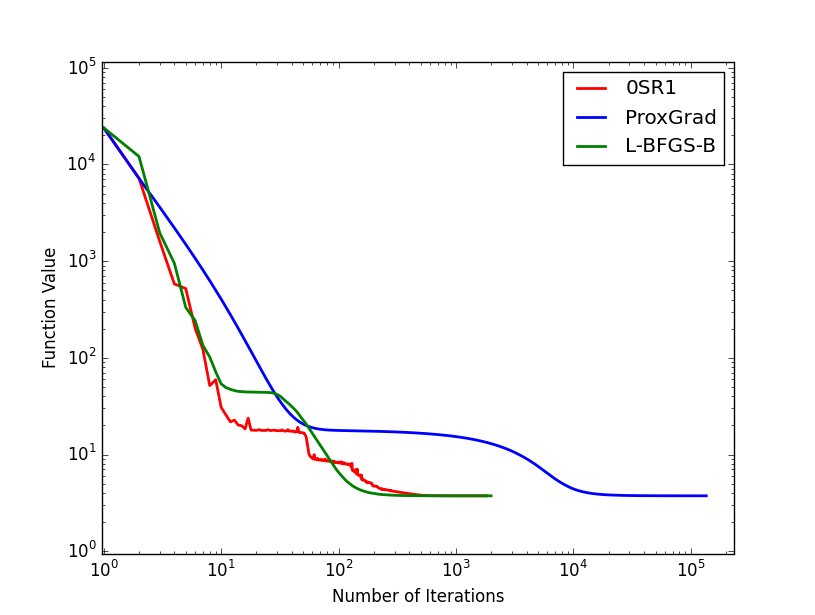
\includegraphics[width = 0.9\textwidth]{ProxNormal_full.png}
\end{frame}
\begin{frame}{Proximal Method}
	\begin{columns}[T]
		\begin{column}{.5\textwidth}
			$F(x) = \lVert Ax - b \rVert + \lambda \lVert x \rVert_1$\\
			$A \in \mathbb{R}^{1500 \times 3000},\:b \in \mathbb{R}^{1500}$\\
			$A_{ij},\:b_i\:$ \textasciitilde $\:\mathcal{N}(0,1)$, $\:\lambda = 0.1$\\
			\vspace{28pt}
			\resizebox{\linewidth}{!}{% This file was created by matplotlib v0.1.0.
% Copyright (c) 2010--2014, Nico Schl�mer <nico.schloemer@gmail.com>
% All rights reserved.
% 
% The lastest updates can be retrieved from
% 
% https://github.com/nschloe/matplotlib2tikz
% 
% where you can also submit bug reports and leavecomments.
% 
\begin{tikzpicture}

\begin{axis}[
xlabel={Number of Iterations},
ylabel={Convergence Factor},
xmin=0, xmax=20,
ymin=0, ymax=1.2,
axis on top,
legend entries={{0SR1},{ProxGrad},{L-BFGS-B}}
]
\addplot [thick, red]
coordinates {
(0,0.848084289429647)
(1,0.571531400706569)
(2,0.3183225225932)
(3,0.325478497212272)
(4,0.229202978836947)
(5,0)

};
\addplot [thick, blue]
coordinates {
(0,0.848084289429647)
(1,0.8761766786044)
(2,0.880353893444499)
(3,0.87631111105461)
(4,0.86750215311503)
(5,0.854873771332014)
(6,0.838545313511358)
(7,0.818309544143084)
(8,0.79368954997227)
(9,0.764405434650521)
(10,0.730785088934228)
(11,0.693056976527169)
(12,0.648410891181648)
(13,0.596467221748105)
(14,0.534977444909731)
(15,0.437803770596474)
(16,0.237479072114323)
(17,0)

};
\addplot [thick, green!50.0!black]
coordinates {
(0,1.03508957652092)
(1,0.953934356298228)
(2,0.781748660719143)
(3,0.348075428829538)
(4,0.392758852840426)
(5,0.321571723894868)
(6,0.494833621279672)
(7,0.62180136584259)
(8,0.66911034267718)
(9,0)

};
\path [draw=black, fill opacity=0] (axis cs:13,0)--(axis cs:13,0);

\path [draw=black, fill opacity=0] (axis cs:13,1)--(axis cs:13,1);

\path [draw=black, fill opacity=0] (axis cs:0,13)--(axis cs:0,13);

\path [draw=black, fill opacity=0] (axis cs:1,13)--(axis cs:1,13);

\end{axis}

\end{tikzpicture}}
		\end{column}\hfill
		\begin{column}{.5\textwidth}
			$F(x) = \lVert Ax - b \rVert + \lambda \lVert x \rVert_1$\\
			$A \in \mathbb{R}^{2197 \times 2197},\:b \in \mathbb{R}^{2197}$\\
			$A$: \small Discretization of 3D Laplacian\\
			\normalsize$\lambda = 1$\\
			\vspace{10pt}
			\resizebox{\linewidth}{!}{% This file was created by matplotlib v0.1.0.
% Copyright (c) 2010--2014, Nico Schl�mer <nico.schloemer@gmail.com>
% All rights reserved.
% 
% The lastest updates can be retrieved from
% 
% https://github.com/nschloe/matplotlib2tikz
% 
% where you can also submit bug reports and leavecomments.
% 
\begin{tikzpicture}

\begin{axis}[
xlabel={Number of Iterations},
ylabel={Convergence Factor},
xmin=0, xmax=20,
ymin=0, ymax=1.2,
axis on top,
legend entries={{0SR1},{ProxGrad},{L-BFGS-B}}
]
\addplot [thick, red]
coordinates {
(0,0.848084289429647)
(1,0.571531400706569)
(2,0.3183225225932)
(3,0.325478497212281)
(4,0.229202978836935)
(5,0)

};
\addplot [thick, blue]
coordinates {
(0,0.848084289429647)
(1,0.8761766786044)
(2,0.880353893444499)
(3,0.87631111105461)
(4,0.86750215311503)
(5,0.854873771332013)
(6,0.838545313511358)
(7,0.818309544143084)
(8,0.79368954997227)
(9,0.764405434650521)
(10,0.730785088934228)
(11,0.693056976527169)
(12,0.648410891181648)
(13,0.596467221748105)
(14,0.534977444909731)
(15,0.437803770596473)
(16,0.237479072114322)
(17,0)

};
\addplot [thick, green!50.0!black]
coordinates {
(0,1.03508957652092)
(1,0.953934356298228)
(2,0.781748660719143)
(3,0.348075428829538)
(4,0.392758852840426)
(5,0.321571723894868)
(6,0.494833621279672)
(7,0.62180136584259)
(8,0.66911034267718)
(9,0)

};
\path [draw=black, fill opacity=0] (axis cs:13,0)--(axis cs:13,0);

\path [draw=black, fill opacity=0] (axis cs:13,1)--(axis cs:13,1);

\path [draw=black, fill opacity=0] (axis cs:0,13)--(axis cs:0,13);

\path [draw=black, fill opacity=0] (axis cs:1,13)--(axis cs:1,13);

\end{axis}

\end{tikzpicture}}
		\end{column}
	\end{columns}
\end{frame}

\begin{frame}{Proximal Method}
	\centering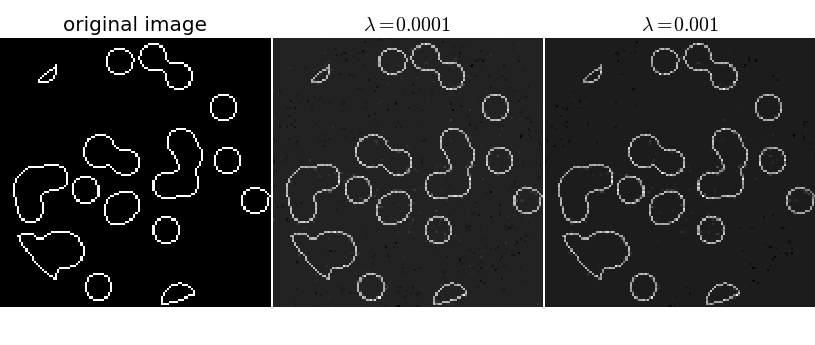
\includegraphics[width=0.9\textwidth]{lambda1.png}\\
	\centering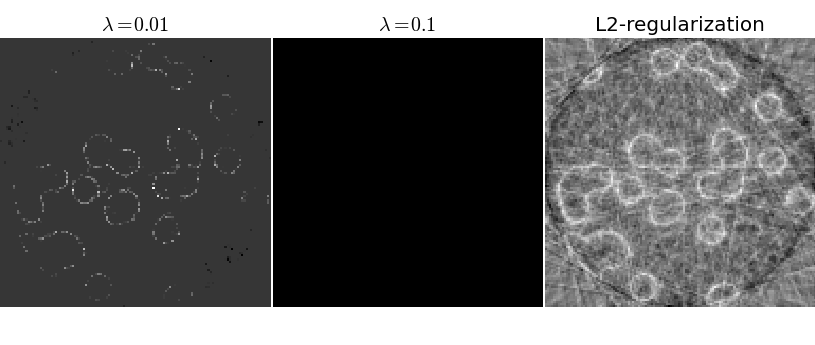
\includegraphics[width=0.9\textwidth]{lambda2.png}

\end{frame}


\begin{frame}
	\begin{figure}[h!]
		\centering
		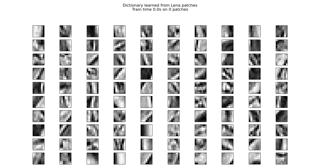
\includegraphics[scale=0.25]{lena_dictionary.png}
		\caption{Dictionary learned}
	\end{figure}
	
\end{frame}
\end{document}
